\pdfminorversion=6 % this is needed to be able to include pdf 1.6. 
                    % For some reasons some old HPSG proceedings have pdf 1.6
\documentclass[11pt,a4paper,fleqn]{article}
\usepackage{times}
\thispagestyle{empty}



\usepackage[T1]{fontenc}   % Silbentrennung

\usepackage[utf8x]{inputenc}
                                                                                                                             
\hyphenation{Acad-e-my}

\usepackage[bookmarks=true,bookmarksopen=true,%
breaklinks=true,%
draft=false,plainpages=false,hyperfootnotes=false,%
pdfauthor={Stefan Müller (Editor)},%
pdftitle={Proceedings of the 12th International Conference on Head-Driven Phrase Structure Grammar},%
pdfkeywords={HPSG}%,
pdftex=true%
%ps2pdf=true  %ohne diesen Treiber geht der Zeilenumbruch in URLs
]{hyperref}% for pdf files
\hypersetup{colorlinks=false, pdfborder={0 0 0}}

\usepackage{pdfpages}
\pdfinclusioncopyfonts=1

\newcommand\formatauthor[2]{\begin{tabular}[t]{@{}c@{}}
  {\LARGE#1\strut}\\
  {\small#2\strut}\\
  \rule{\dimexpr0.5\linewidth-1em}{0pt}
  \end{tabular}\xhfill\ignorespaces}
\newcommand\xhfill{\hspace{1em plus 1fill}}

\begin{document}

\begin{center}
{\Large
                {\bfseries Proceedings of the 12th International Conference on\par Head-Driven Phrase Structure Grammar\par}

                \vspace{8ex}

                     Department of Informatics, University of Lisbon\\[\baselineskip]

                        Stefan M{\"u}ller (Editor)\\[\baselineskip]

                                2005\\[\baselineskip]

                          CSLI Publications\\[\baselineskip]

              http://csli-publications.stanford.edu/HPSG/2005 \\[4\baselineskip]

The papers are published under a \href{http://creativecommons.org/licenses/by/4.0/}{CC-BY license}:\\[3pt]
\href{http://creativecommons.org/licenses/by/4.0/}{http://creativecommons.org/licenses/by/4.0/}
}
\end{center}
\newpage
\tableofcontents

\newpage

\section{Editor's Note}
The 12th International Conference on Head-Driven Phrase Structure Grammar (2005) was held at
the Department of Informatics, University of Lisbon in Portugal.

The conference featured 2 invited talks, 18 papers, 2 alternate papers, and 6 posters
selected by the program committee 
(Raul Aranovich,
Doug Arnold,
Emily Bender,
Olivier Bonami,
António Branco,
Berthold Crysmann,
Anke Holler,
Valia Kordoni,
Palmira Marrafa,
Tsuneko Nakazawa,
Gerald Penn,
Alexander Rosen,
Manfred Sailer (chair),
Gautam Sengupta,
Jesse Tseng,
Stephen Wechsler, and
Shuly Winter). 
A workshop on \emph{Binding Theory and Invariants in Anaphoric Relations} was attached to the conference. It featured one invited talk
and 12 papers, selected by the workshop program committee (Pilar Barbosa,
António Branco (chair),
Rejean Canac-Marquis,
Mary Dalrymple,
Martin Evearert,
Volker Gast,
Lars Hellan,
Ehrard Hinrichs,
Yan Huang,
Tibor Kiss,
Frank Keller,
Valia Kordoni,
Maria Pinango,
Carl Pollard,
Janina Radó,
Eric Reuland,
Jeffrey Runner,
Ivan Sag,
Roland Stuckardt,
Ping Xue).

In total there were 39 submissions to the main conference and 13 submissions to the
workshop. 
We want to thank the respective program committees for putting this nice program together.

Thanks go to António Branco, who was in charge of local arrangements.

As in the past years the contributions to the conference proceedings are based on the five page abstract
that was reviewed by the respective program committees, but there is no additional reviewing of the
longer contribution to the proceedings.
To ensure easy access and fast publication we have chosen an electronic format.

The proceedings include all the papers except those by 
Frank Keller and Theodora Alexopoulou, Stefan Müller and Eric Reuland. Nurit Melnik submitted
an extended abstract, the full paper will appear in a Research on Language and Computation.


\newpage
\part{Contributions to the Main Conference}
\thispagestyle{empty}
\newpage
        \setcounter{page}{7}
        \phantomsection
        \addcontentsline{toc}{section}{Douglas Ball: Tongan Noun Incorporation: Lexical Sharing or Argument Inheritance}
\thispagestyle{empty}

\begin{center}
  {\huge\bfseries Tongan Noun Incorporation: Lexical Sharing or Argument Inheritance\par}

  \bigskip

~\\
\begingroup
\setlength{\leftskip}{0pt plus 1fill}
\setlength{\rightskip}{0pt plus 1fill}
\setlength{\parindent}{0pt}
\setlength{\parfillskip}{0pt}
  \formatauthor{Douglas Ball}{\begin{tabular}{@{}c@{}}Stanford University\end{tabular}}

\par\endgroup

  \vspace*{8ex}

  Proceedings of the 12th International Conference on\par Head-Driven Phrase Structure Grammar

  \bigskip

  Department of Informatics, University of Lisbon

  \medskip

  Stefan Müller (Editor)

  \medskip

  2005

  \medskip

  CSLI Publications

  \medskip

  pages 7--27

  \medskip

  \url{http://csli-publications.stanford.edu/HPSG/2005}
\end{center}
\vfill

\noindent



\vfill
\noindent
% APA Style
Ball, Douglas. 2005. Tongan Noun Incorporation: Lexical Sharing or Argument Inheritance. In Müller, Stefan (Ed.), \emph{{Proceedings of the 12th International Conference on Head-Driven Phrase Structure Grammar, Department of Informatics, University of Lisbon}}, 7--27. Stanford,
CA: CSLI Publications. \hfill\href{http://creativecommons.org/licenses/by/4.0/}{\includegraphics[height=.75em]{Includes/ccby.eps}}

\newpage
\includepdf[pages=-,pagecommand=\thispagestyle{plain}]{Includes/ball.pdf}
        \setcounter{page}{28}
        \phantomsection
        \addcontentsline{toc}{section}{John Beavers: Towards A Semantic Analysis of Argument/Oblique Alternations in HPSG}
\thispagestyle{empty}

\begin{center}
  {\huge\bfseries Towards A Semantic Analysis of Argument/Oblique Alternations in HPSG\par}

  \bigskip

~\\
\begingroup
\setlength{\leftskip}{0pt plus 1fill}
\setlength{\rightskip}{0pt plus 1fill}
\setlength{\parindent}{0pt}
\setlength{\parfillskip}{0pt}
  \formatauthor{John Beavers}{\begin{tabular}{@{}c@{}}CSLI, Stanford University\end{tabular}}

\par\endgroup

  \vspace*{8ex}

  Proceedings of the 12th International Conference on\par Head-Driven Phrase Structure Grammar

  \bigskip

  Department of Informatics, University of Lisbon

  \medskip

  Stefan Müller (Editor)

  \medskip

  2005

  \medskip

  CSLI Publications

  \medskip

  pages 28--48

  \medskip

  \url{http://csli-publications.stanford.edu/HPSG/2005}
\end{center}
\vfill

\noindent



\vfill
\noindent
% APA Style
Beavers, John. 2005. Towards A Semantic Analysis of Argument/Oblique Alternations in HPSG. In Müller, Stefan (Ed.), \emph{{Proceedings of the 12th International Conference on Head-Driven Phrase Structure Grammar, Department of Informatics, University of Lisbon}}, 28--48. Stanford,
CA: CSLI Publications. \hfill\href{http://creativecommons.org/licenses/by/4.0/}{\includegraphics[height=.75em]{Includes/ccby.eps}}

\newpage
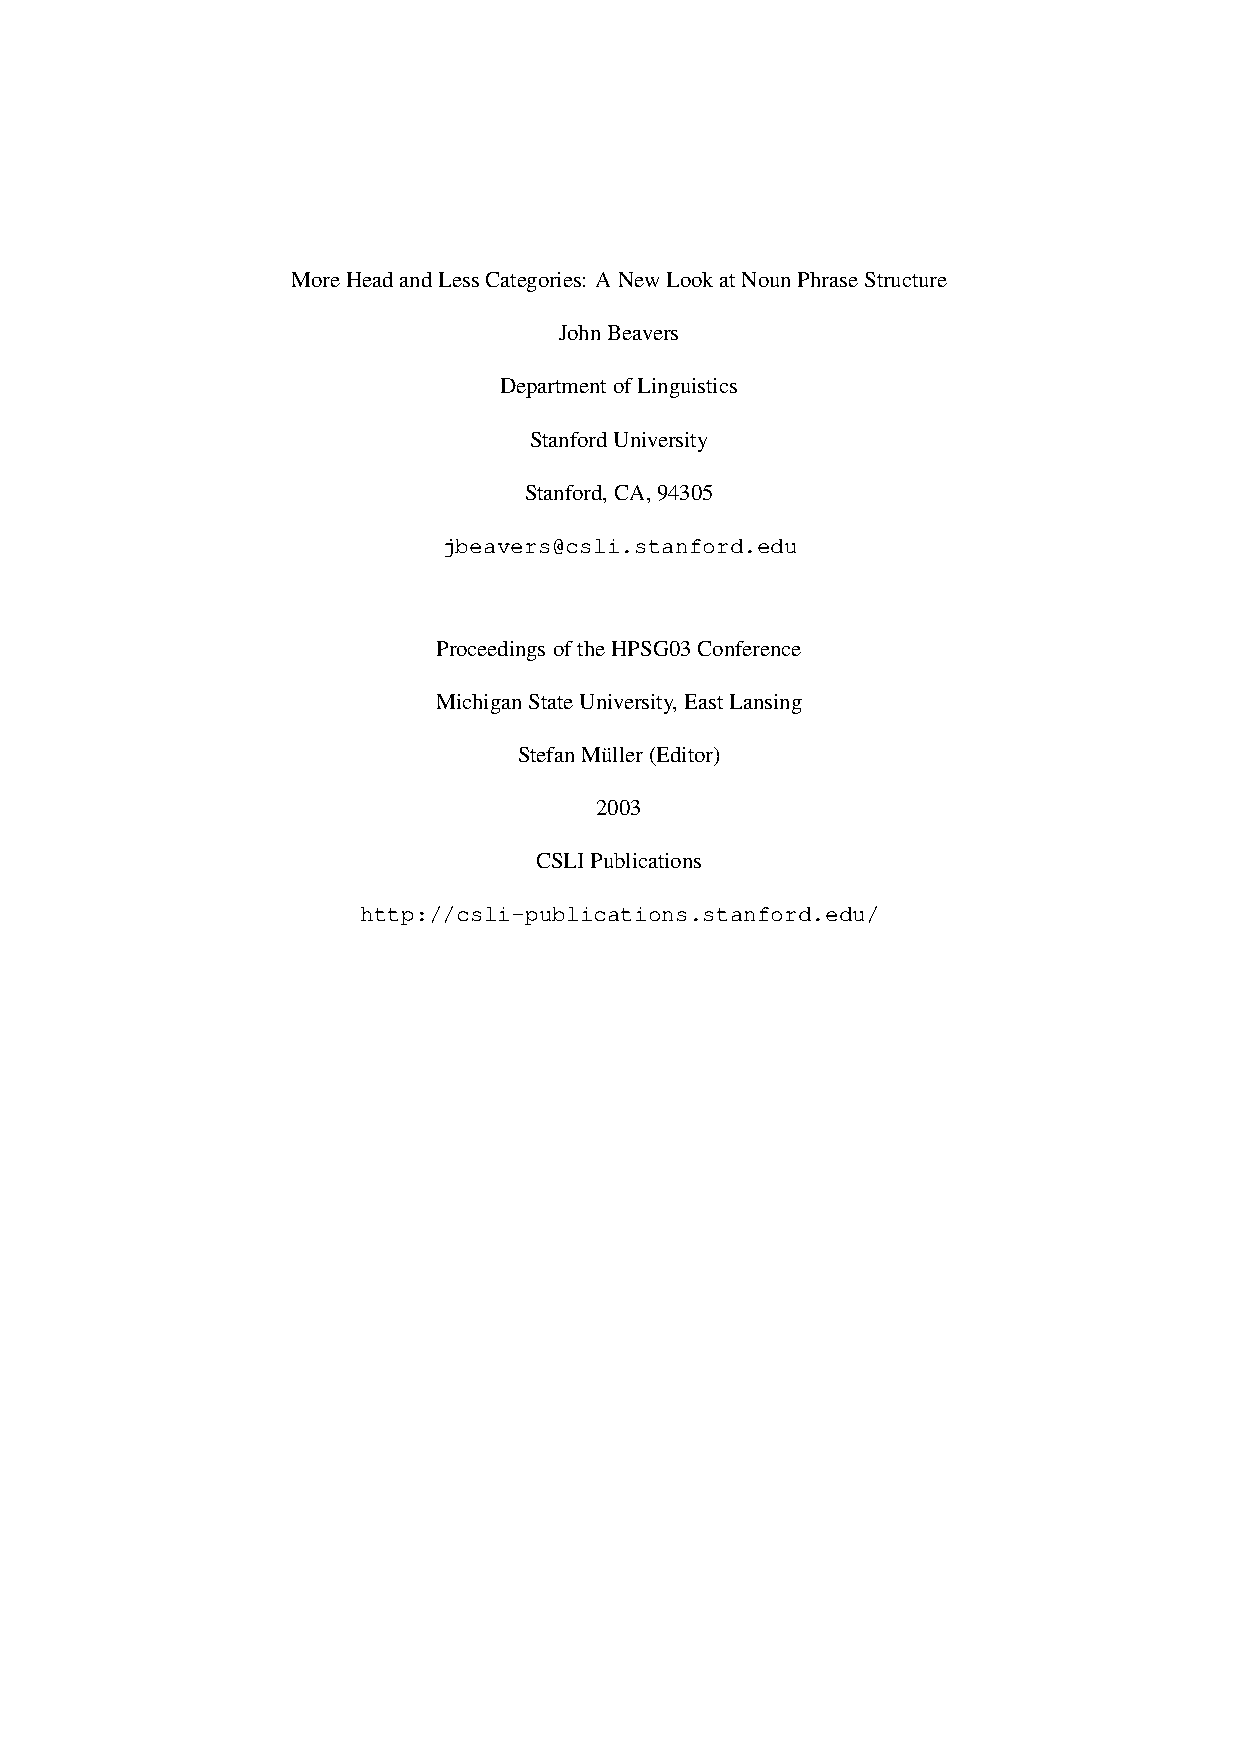
\includepdf[pages=-,pagecommand=\thispagestyle{plain}]{Includes/beavers.pdf}
        \setcounter{page}{49}
        \phantomsection
        \addcontentsline{toc}{section}{Núria Bertomeu, Valia Kordoni: Integrating Pragmatic Information in  Grammar. An Analysis of Intersentential Ellipsis}
\thispagestyle{empty}

\begin{center}
  {\huge\bfseries Integrating Pragmatic Information in  Grammar. An Analysis of Intersentential Ellipsis\par}

  \bigskip

~\\
\begingroup
\setlength{\leftskip}{0pt plus 1fill}
\setlength{\rightskip}{0pt plus 1fill}
\setlength{\parindent}{0pt}
\setlength{\parfillskip}{0pt}
  \formatauthor{Núria Bertomeu}{\begin{tabular}{@{}c@{}}Saarland University\end{tabular}}
\formatauthor{Valia Kordoni}{\begin{tabular}{@{}c@{}}Saarland University\end{tabular}}

\par\endgroup

  \vspace*{8ex}

  Proceedings of the 12th International Conference on\par Head-Driven Phrase Structure Grammar

  \bigskip

  Department of Informatics, University of Lisbon

  \medskip

  Stefan Müller (Editor)

  \medskip

  2005

  \medskip

  CSLI Publications

  \medskip

  pages 49--69

  \medskip

  \url{http://csli-publications.stanford.edu/HPSG/2005}
\end{center}
\vfill

\noindent



\vfill
\noindent
% APA Style
Bertomeu, Núria, \& Kordoni, Valia. 2005. Integrating Pragmatic Information in  Grammar. An Analysis of Intersentential Ellipsis. In Müller, Stefan (Ed.), \emph{{Proceedings of the 12th International Conference on Head-Driven Phrase Structure Grammar, Department of Informatics, University of Lisbon}}, 49--69. Stanford,
CA: CSLI Publications. \hfill\href{http://creativecommons.org/licenses/by/4.0/}{\includegraphics[height=.75em]{Includes/ccby.eps}}

\newpage
\includepdf[pages=-,pagecommand=\thispagestyle{plain}]{Includes/bertomeu-kordoni.pdf}
        \setcounter{page}{70}
        \phantomsection
        \addcontentsline{toc}{section}{Denis Creissels, Dani\`{e}le Godard: The Tswana Infinitive as a Mixed Category}
\thispagestyle{empty}

\begin{center}
  {\huge\bfseries The Tswana Infinitive as a Mixed Category\par}

  \bigskip

~\\
\begingroup
\setlength{\leftskip}{0pt plus 1fill}
\setlength{\rightskip}{0pt plus 1fill}
\setlength{\parindent}{0pt}
\setlength{\parfillskip}{0pt}
  \formatauthor{Denis Creissels}{\begin{tabular}{@{}c@{}}Université Lyon 2\end{tabular}}
\formatauthor{Danièle Godard}{\begin{tabular}{@{}c@{}}CNRS et U. Paris 7\end{tabular}}

\par\endgroup

  \vspace*{8ex}

  Proceedings of the 12th International Conference on\par Head-Driven Phrase Structure Grammar

  \bigskip

  Department of Informatics, University of Lisbon

  \medskip

  Stefan Müller (Editor)

  \medskip

  2005

  \medskip

  CSLI Publications

  \medskip

  pages 70--90

  \medskip

  \url{http://csli-publications.stanford.edu/HPSG/2005}
\end{center}
\vfill

\noindent



\vfill
\noindent
% APA Style
Creissels, Denis, \& Godard, Danièle. 2005. The Tswana Infinitive as a Mixed Category. In Müller, Stefan (Ed.), \emph{{Proceedings of the 12th International Conference on Head-Driven Phrase Structure Grammar, Department of Informatics, University of Lisbon}}, 70--90. Stanford,
CA: CSLI Publications. \hfill\href{http://creativecommons.org/licenses/by/4.0/}{\includegraphics[height=.75em]{Includes/ccby.eps}}

\newpage
\includepdf[pages=-,pagecommand=\thispagestyle{plain}]{Includes/creissels-godard.pdf}
        \setcounter{page}{91}
        \phantomsection
        \addcontentsline{toc}{section}{Berthold Crysmann: Syncretism in German: A Unified Approach to Underspecification, Indeterminacy, and Likeness of Case}
\thispagestyle{empty}

\begin{center}
  {\huge\bfseries Syncretism in German: A Unified Approach to Underspecification, Indeterminacy, and Likeness of Case\par}

  \bigskip

~\\
\begingroup
\setlength{\leftskip}{0pt plus 1fill}
\setlength{\rightskip}{0pt plus 1fill}
\setlength{\parindent}{0pt}
\setlength{\parfillskip}{0pt}
  \formatauthor{Berthold Crysmann}{\begin{tabular}{@{}c@{}}Universität des Saarlandes\end{tabular}}

\par\endgroup

  \vspace*{8ex}

  Proceedings of the 12th International Conference on\par Head-Driven Phrase Structure Grammar

  \bigskip

  Department of Informatics, University of Lisbon

  \medskip

  Stefan Müller (Editor)

  \medskip

  2005

  \medskip

  CSLI Publications

  \medskip

  pages 91--107

  \medskip

  \url{http://csli-publications.stanford.edu/HPSG/2005}
\end{center}
\vfill

\noindent



\vfill
\noindent
% APA Style
Crysmann, Berthold. 2005. Syncretism in German: A Unified Approach to Underspecification, Indeterminacy, and Likeness of Case. In Müller, Stefan (Ed.), \emph{{Proceedings of the 12th International Conference on Head-Driven Phrase Structure Grammar, Department of Informatics, University of Lisbon}}, 91--107. Stanford,
CA: CSLI Publications. \hfill\href{http://creativecommons.org/licenses/by/4.0/}{\includegraphics[height=.75em]{Includes/ccby.eps}}

\newpage
\includepdf[pages=-,pagecommand=\thispagestyle{plain}]{Includes/crysmann.pdf}
        \setcounter{page}{108}
        \phantomsection
        \addcontentsline{toc}{section}{Scott Drellishak, Emily M. Bender: A Coordination Module for a Crosslinguistic Grammar Resource}
\thispagestyle{empty}

\begin{center}
  {\huge\bfseries A Coordination Module for a Crosslinguistic Grammar Resource\par}

  \bigskip

~\\
\begingroup
\setlength{\leftskip}{0pt plus 1fill}
\setlength{\rightskip}{0pt plus 1fill}
\setlength{\parindent}{0pt}
\setlength{\parfillskip}{0pt}
  \formatauthor{Scott Drellishak}{\begin{tabular}{@{}c@{}}University of Washington\end{tabular}}
\formatauthor{Emily M. Bender}{\begin{tabular}{@{}c@{}}University of Washington\end{tabular}}

\par\endgroup

  \vspace*{8ex}

  Proceedings of the 12th International Conference on\par Head-Driven Phrase Structure Grammar

  \bigskip

  Department of Informatics, University of Lisbon

  \medskip

  Stefan Müller (Editor)

  \medskip

  2005

  \medskip

  CSLI Publications

  \medskip

  pages 108--128

  \medskip

  \url{http://csli-publications.stanford.edu/HPSG/2005}
\end{center}
\vfill

\noindent



\vfill
\noindent
% APA Style
Drellishak, Scott, \& Bender, Emily M. 2005. A Coordination Module for a Crosslinguistic Grammar Resource. In Müller, Stefan (Ed.), \emph{{Proceedings of the 12th International Conference on Head-Driven Phrase Structure Grammar, Department of Informatics, University of Lisbon}}, 108--128. Stanford,
CA: CSLI Publications. \hfill\href{http://creativecommons.org/licenses/by/4.0/}{\includegraphics[height=.75em]{Includes/ccby.eps}}

\newpage
\includepdf[pages=-,pagecommand=\thispagestyle{plain}]{Includes/drellishak-bender.pdf}
        \setcounter{page}{129}
        \phantomsection
        \addcontentsline{toc}{section}{Dan Flickinger, Alexander Koller, Stafan Thater: A New Well-Formedness Criterion for Semantics Debugging}
\thispagestyle{empty}

\begin{center}
  {\huge\bfseries A New Well-Formedness Criterion for Semantics Debugging\par}

  \bigskip

~\\
\begingroup
\setlength{\leftskip}{0pt plus 1fill}
\setlength{\rightskip}{0pt plus 1fill}
\setlength{\parindent}{0pt}
\setlength{\parfillskip}{0pt}
  \formatauthor{Dan Flickinger}{\begin{tabular}{@{}c@{}}Stanford University\end{tabular}}
\formatauthor{Alexander Koller}{\begin{tabular}{@{}c@{}}Universität des Saarlands\end{tabular}}
\formatauthor{Stafan Thater}{\begin{tabular}{@{}c@{}}Universität des Saarlands\end{tabular}}

\par\endgroup

  \vspace*{8ex}

  Proceedings of the 12th International Conference on\par Head-Driven Phrase Structure Grammar

  \bigskip

  Department of Informatics, University of Lisbon

  \medskip

  Stefan Müller (Editor)

  \medskip

  2005

  \medskip

  CSLI Publications

  \medskip

  pages 129--142

  \medskip

  \url{http://csli-publications.stanford.edu/HPSG/2005}
\end{center}
\vfill

\noindent



\vfill
\noindent
% APA Style
Flickinger, Dan, Koller, Alexander, \& Thater, Stafan. 2005. A New Well-Formedness Criterion for Semantics Debugging. In Müller, Stefan (Ed.), \emph{{Proceedings of the 12th International Conference on Head-Driven Phrase Structure Grammar, Department of Informatics, University of Lisbon}}, 129--142. Stanford,
CA: CSLI Publications. \hfill\href{http://creativecommons.org/licenses/by/4.0/}{\includegraphics[height=.75em]{Includes/ccby.eps}}

\newpage
\includepdf[pages=-,pagecommand=\thispagestyle{plain}]{Includes/fkt.pdf}
        \setcounter{page}{143}
        \phantomsection
        \addcontentsline{toc}{section}{Chikara Hashimoto, Francis Bond: A Computational Treatment of V-V Compounds in Japanese}
\thispagestyle{empty}

\begin{center}
  {\huge\bfseries A Computational Treatment of V-V Compounds in Japanese\par}

  \bigskip

~\\
\begingroup
\setlength{\leftskip}{0pt plus 1fill}
\setlength{\rightskip}{0pt plus 1fill}
\setlength{\parindent}{0pt}
\setlength{\parfillskip}{0pt}
  \formatauthor{Chikara Hashimoto}{\begin{tabular}{@{}c@{}}Kyoto University\end{tabular}}
\formatauthor{Francis Bond}{\begin{tabular}{@{}c@{}}NTT Communication Science Laboratories\end{tabular}}

\par\endgroup

  \vspace*{8ex}

  Proceedings of the 12th International Conference on\par Head-Driven Phrase Structure Grammar

  \bigskip

  Department of Informatics, University of Lisbon

  \medskip

  Stefan Müller (Editor)

  \medskip

  2005

  \medskip

  CSLI Publications

  \medskip

  pages 143--156

  \medskip

  \url{http://csli-publications.stanford.edu/HPSG/2005}
\end{center}
\vfill

\noindent



\vfill
\noindent
% APA Style
Hashimoto, Chikara, \& Bond, Francis. 2005. A Computational Treatment of V-V Compounds in Japanese. In Müller, Stefan (Ed.), \emph{{Proceedings of the 12th International Conference on Head-Driven Phrase Structure Grammar, Department of Informatics, University of Lisbon}}, 143--156. Stanford,
CA: CSLI Publications. \hfill\href{http://creativecommons.org/licenses/by/4.0/}{\includegraphics[height=.75em]{Includes/ccby.eps}}

\newpage
\includepdf[pages=-,pagecommand=\thispagestyle{plain}]{Includes/hashimoto-bond.pdf}
        \setcounter{page}{157}
        \phantomsection
        \addcontentsline{toc}{section}{Anke Holler: On Non-Canonical Clause Linkage}
\thispagestyle{empty}

\begin{center}
  {\huge\bfseries On Non-Canonical Clause Linkage\par}

  \bigskip

~\\
\begingroup
\setlength{\leftskip}{0pt plus 1fill}
\setlength{\rightskip}{0pt plus 1fill}
\setlength{\parindent}{0pt}
\setlength{\parfillskip}{0pt}
  \formatauthor{Anke Holler}{\begin{tabular}{@{}c@{}}University of Heidelberg\end{tabular}}

\par\endgroup

  \vspace*{8ex}

  Proceedings of the 12th International Conference on\par Head-Driven Phrase Structure Grammar

  \bigskip

  Department of Informatics, University of Lisbon

  \medskip

  Stefan Müller (Editor)

  \medskip

  2005

  \medskip

  CSLI Publications

  \medskip

  pages 157--177

  \medskip

  \url{http://csli-publications.stanford.edu/HPSG/2005}
\end{center}
\vfill

\noindent



\vfill
\noindent
% APA Style
Holler, Anke. 2005. On Non-Canonical Clause Linkage. In Müller, Stefan (Ed.), \emph{{Proceedings of the 12th International Conference on Head-Driven Phrase Structure Grammar, Department of Informatics, University of Lisbon}}, 157--177. Stanford,
CA: CSLI Publications. \hfill\href{http://creativecommons.org/licenses/by/4.0/}{\includegraphics[height=.75em]{Includes/ccby.eps}}

\newpage
\includepdf[pages=-,pagecommand=\thispagestyle{plain}]{Includes/holler.pdf}
        \setcounter{page}{178}
        \phantomsection
        \addcontentsline{toc}{section}{Christopher Kennedy, Louise McNally: The Syntax and Semantics of Multiple Degree Modification in English}
\thispagestyle{empty}

\begin{center}
  {\huge\bfseries The Syntax and Semantics of Multiple Degree Modification in English\par}

  \bigskip

~\\
\begingroup
\setlength{\leftskip}{0pt plus 1fill}
\setlength{\rightskip}{0pt plus 1fill}
\setlength{\parindent}{0pt}
\setlength{\parfillskip}{0pt}
  \formatauthor{Christopher Kennedy}{\begin{tabular}{@{}c@{}}University of Chicago\end{tabular}}
\formatauthor{Louise McNally}{\begin{tabular}{@{}c@{}}Universitat Pompeu Fabra\end{tabular}}

\par\endgroup

  \vspace*{8ex}

  Proceedings of the 12th International Conference on\par Head-Driven Phrase Structure Grammar

  \bigskip

  Department of Informatics, University of Lisbon

  \medskip

  Stefan Müller (Editor)

  \medskip

  2005

  \medskip

  CSLI Publications

  \medskip

  pages 178--191

  \medskip

  \url{http://csli-publications.stanford.edu/HPSG/2005}
\end{center}
\vfill

\noindent



\vfill
\noindent
% APA Style
Kennedy, Christopher, \& McNally,  Louise. 2005. The Syntax and Semantics of Multiple Degree Modification in English. In Müller, Stefan (Ed.), \emph{{Proceedings of the 12th International Conference on Head-Driven Phrase Structure Grammar, Department of Informatics, University of Lisbon}}, 178--191. Stanford,
CA: CSLI Publications. \hfill\href{http://creativecommons.org/licenses/by/4.0/}{\includegraphics[height=.75em]{Includes/ccby.eps}}

\newpage
\includepdf[pages=-,pagecommand=\thispagestyle{plain}]{Includes/kennedy-mcnally.pdf}
        \setcounter{page}{192}
        \phantomsection
        \addcontentsline{toc}{section}{Jong-Bok Kim, Ivan A. Sag: English Object Extraposition:\\ A Constraint-Based Approach}
\thispagestyle{empty}

\begin{center}
  {\huge\bfseries English Object Extraposition:\par A Constraint-Based Approach\par}

  \bigskip

~\\
\begingroup
\setlength{\leftskip}{0pt plus 1fill}
\setlength{\rightskip}{0pt plus 1fill}
\setlength{\parindent}{0pt}
\setlength{\parfillskip}{0pt}
  \formatauthor{Jong-Bok Kim}{\begin{tabular}{@{}c@{}}Kyung Hee University\end{tabular}}
\formatauthor{Ivan A. Sag}{\begin{tabular}{@{}c@{}}Stanford University\end{tabular}}

\par\endgroup

  \vspace*{8ex}

  Proceedings of the 12th International Conference on\par Head-Driven Phrase Structure Grammar

  \bigskip

  Department of Informatics, University of Lisbon

  \medskip

  Stefan Müller (Editor)

  \medskip

  2005

  \medskip

  CSLI Publications

  \medskip

  pages 192--212

  \medskip

  \url{http://csli-publications.stanford.edu/HPSG/2005}
\end{center}
\vfill

\noindent



\vfill
\noindent
% APA Style
Kim, Jong-Bok, \& Sag, Ivan A. 2005. English Object Extraposition:  A Constraint-Based Approach. In Müller, Stefan (Ed.), \emph{{Proceedings of the 12th International Conference on Head-Driven Phrase Structure Grammar, Department of Informatics, University of Lisbon}}, 192--212. Stanford,
CA: CSLI Publications. \hfill\href{http://creativecommons.org/licenses/by/4.0/}{\includegraphics[height=.75em]{Includes/ccby.eps}}

\newpage
\includepdf[pages=-,pagecommand=\thispagestyle{plain}]{Includes/kim-sag.pdf}
        \setcounter{page}{213}
        \phantomsection
        \addcontentsline{toc}{section}{Jong-Bok Kim, Peter Sells: Copy Constructions and their Interaction with the Copula in Korean}
\thispagestyle{empty}

\begin{center}
  {\huge\bfseries Copy Constructions and their Interaction with the Copula in Korean\par}

  \bigskip

~\\
\begingroup
\setlength{\leftskip}{0pt plus 1fill}
\setlength{\rightskip}{0pt plus 1fill}
\setlength{\parindent}{0pt}
\setlength{\parfillskip}{0pt}
  \formatauthor{Jong-Bok Kim}{\begin{tabular}{@{}c@{}}Kyung Hee University\end{tabular}}
\formatauthor{Peter Sells}{\begin{tabular}{@{}c@{}}Stanford University\end{tabular}}

\par\endgroup

  \vspace*{8ex}

  Proceedings of the 12th International Conference on\par Head-Driven Phrase Structure Grammar

  \bigskip

  Department of Informatics, University of Lisbon

  \medskip

  Stefan Müller (Editor)

  \medskip

  2005

  \medskip

  CSLI Publications

  \medskip

  pages 213--231

  \medskip

  \url{http://csli-publications.stanford.edu/HPSG/2005}
\end{center}
\vfill

\noindent



\vfill
\noindent
% APA Style
Kim, Jong-Bok, \& Sells, Peter. 2005. Copy Constructions and their Interaction with the Copula in Korean. In Müller, Stefan (Ed.), \emph{{Proceedings of the 12th International Conference on Head-Driven Phrase Structure Grammar, Department of Informatics, University of Lisbon}}, 213--231. Stanford,
CA: CSLI Publications. \hfill\href{http://creativecommons.org/licenses/by/4.0/}{\includegraphics[height=.75em]{Includes/ccby.eps}}

\newpage
\includepdf[pages=-,pagecommand=\thispagestyle{plain}]{Includes/kim-sells.pdf}
        \setcounter{page}{232}
        \phantomsection
        \addcontentsline{toc}{section}{Yusuke Kubota: Toward a Unified Analysis of the Scope Interpretation of Complex}
\thispagestyle{empty}

\begin{center}
  {\huge\bfseries Toward a Unified Analysis of the Scope Interpretation of Complex\par}

  \bigskip

~\\
\begingroup
\setlength{\leftskip}{0pt plus 1fill}
\setlength{\rightskip}{0pt plus 1fill}
\setlength{\parindent}{0pt}
\setlength{\parfillskip}{0pt}
  \formatauthor{Yusuke Kubota}{\begin{tabular}{@{}c@{}}Ohio State University\end{tabular}}

\par\endgroup

  \vspace*{8ex}

  Proceedings of the 12th International Conference on\par Head-Driven Phrase Structure Grammar

  \bigskip

  Department of Informatics, University of Lisbon

  \medskip

  Stefan Müller (Editor)

  \medskip

  2005

  \medskip

  CSLI Publications

  \medskip

  pages 232--252

  \medskip

  \url{http://csli-publications.stanford.edu/HPSG/2005}
\end{center}
\vfill

\noindent



\vfill
\noindent
% APA Style
Kubota, Yusuke. 2005. Toward a Unified Analysis of the Scope Interpretation of Complex. In Müller, Stefan (Ed.), \emph{{Proceedings of the 12th International Conference on Head-Driven Phrase Structure Grammar, Department of Informatics, University of Lisbon}}, 232--252. Stanford,
CA: CSLI Publications. \hfill\href{http://creativecommons.org/licenses/by/4.0/}{\includegraphics[height=.75em]{Includes/ccby.eps}}

\newpage
\includepdf[pages=-,pagecommand=\thispagestyle{plain}]{Includes/kubota.pdf}
        \setcounter{page}{253}
        \phantomsection
        \addcontentsline{toc}{section}{Anna Kup{\'s}{\'c}, Jesse Tseng: A New HPSG Approach to Polish Auxiliary Constructions}
\thispagestyle{empty}

\begin{center}
  {\huge\bfseries A New HPSG Approach to Polish Auxiliary Constructions\par}

  \bigskip

~\\
\begingroup
\setlength{\leftskip}{0pt plus 1fill}
\setlength{\rightskip}{0pt plus 1fill}
\setlength{\parindent}{0pt}
\setlength{\parfillskip}{0pt}
  \formatauthor{Anna Kupść}{\begin{tabular}{@{}c@{}}Polish Academy of Sciences and CNRS, Loria\end{tabular}}
\formatauthor{Jesse Tseng}{\begin{tabular}{@{}c@{}}CNRS, Loria\end{tabular}}

\par\endgroup

  \vspace*{8ex}

  Proceedings of the 12th International Conference on\par Head-Driven Phrase Structure Grammar

  \bigskip

  Department of Informatics, University of Lisbon

  \medskip

  Stefan Müller (Editor)

  \medskip

  2005

  \medskip

  CSLI Publications

  \medskip

  pages 253--273

  \medskip

  \url{http://csli-publications.stanford.edu/HPSG/2005}
\end{center}
\vfill

\noindent



\vfill
\noindent
% APA Style
Kupść, Anna, \& Tseng, Jesse. 2005. A New HPSG Approach to Polish Auxiliary Constructions. In Müller, Stefan (Ed.), \emph{{Proceedings of the 12th International Conference on Head-Driven Phrase Structure Grammar, Department of Informatics, University of Lisbon}}, 253--273. Stanford,
CA: CSLI Publications. \hfill\href{http://creativecommons.org/licenses/by/4.0/}{\includegraphics[height=.75em]{Includes/ccby.eps}}

\newpage
\includepdf[pages=-,pagecommand=\thispagestyle{plain}]{Includes/kupsc-tseng.pdf}
        \setcounter{page}{274}
        \phantomsection
        \addcontentsline{toc}{section}{Sun-Hee Lee: A Trace Analysis of Korean UDCs}
\thispagestyle{empty}

\begin{center}
  {\huge\bfseries A Trace Analysis of Korean UDCs\par}

  \bigskip

~\\
\begingroup
\setlength{\leftskip}{0pt plus 1fill}
\setlength{\rightskip}{0pt plus 1fill}
\setlength{\parindent}{0pt}
\setlength{\parfillskip}{0pt}
  \formatauthor{Sun-Hee Lee}{\begin{tabular}{@{}c@{}}Wellesley College\end{tabular}}

\par\endgroup

  \vspace*{8ex}

  Proceedings of the 12th International Conference on\par Head-Driven Phrase Structure Grammar

  \bigskip

  Department of Informatics, University of Lisbon

  \medskip

  Stefan Müller (Editor)

  \medskip

  2005

  \medskip

  CSLI Publications

  \medskip

  pages 274--289

  \medskip

  \url{http://csli-publications.stanford.edu/HPSG/2005}
\end{center}
\vfill

\noindent
Keywords: 8211; in the traditional HPSG analysis of
UDCs following Pollard and Sag (1994). It is because in HPSG traces 
are not all required to have the same feature, unlike in other
movement-based approaches including the minimalist program and GB
theory. In addition, we argue that the three kinds of Korean UDC
elements appearing in gap positions do not form separate categories
from their corresponding forms appearing in non-UDCs based on the
same semantic and pragmatic properties such as logophoricity and
contrastiveness. We also investigate some controversial issues of
island constraints and strong crossover with respect to filler-gap
linkage in Korean UDCs.


\vfill
\noindent
% APA Style
Lee, Sun-Hee. 2005. A Trace Analysis of Korean UDCs. In Müller, Stefan (Ed.), \emph{{Proceedings of the 12th International Conference on Head-Driven Phrase Structure Grammar, Department of Informatics, University of Lisbon}}, 274--289. Stanford,
CA: CSLI Publications. \hfill\href{http://creativecommons.org/licenses/by/4.0/}{\includegraphics[height=.75em]{Includes/ccby.eps}}

\newpage
\includepdf[pages=-,pagecommand=\thispagestyle{plain}]{Includes/lee.pdf}
        \setcounter{page}{290}
        \phantomsection
        \addcontentsline{toc}{section}{Takafumi Maekawa: An HPSG Approach to the \emph{who}/\emph{whom} Puzzle}
\thispagestyle{empty}

\begin{center}
  {\huge\bfseries An HPSG Approach to the \emph{who}/\emph{whom} Puzzle\par}

  \bigskip

~\\
\begingroup
\setlength{\leftskip}{0pt plus 1fill}
\setlength{\rightskip}{0pt plus 1fill}
\setlength{\parindent}{0pt}
\setlength{\parfillskip}{0pt}
  \formatauthor{Takafumi Maekawa}{\begin{tabular}{@{}c@{}}University of Essex\end{tabular}}

\par\endgroup

  \vspace*{8ex}

  Proceedings of the 12th International Conference on\par Head-Driven Phrase Structure Grammar

  \bigskip

  Department of Informatics, University of Lisbon

  \medskip

  Stefan Müller (Editor)

  \medskip

  2005

  \medskip

  CSLI Publications

  \medskip

  pages 290--310

  \medskip

  \url{http://csli-publications.stanford.edu/HPSG/2005}
\end{center}
\vfill

\noindent



\vfill
\noindent
% APA Style
Maekawa, Takafumi. 2005. An HPSG Approach to the \emph{who}/\emph{whom} Puzzle. In Müller, Stefan (Ed.), \emph{{Proceedings of the 12th International Conference on Head-Driven Phrase Structure Grammar, Department of Informatics, University of Lisbon}}, 290--310. Stanford,
CA: CSLI Publications. \hfill\href{http://creativecommons.org/licenses/by/4.0/}{\includegraphics[height=.75em]{Includes/ccby.eps}}

\newpage
\includepdf[pages=-,pagecommand=\thispagestyle{plain}]{Includes/maekawa.pdf}
        \setcounter{page}{311}
        \phantomsection
        \addcontentsline{toc}{section}{Nurit Melnik: From ``Hand-Written'' to Computationally Implemented HPSG Theories}
\thispagestyle{empty}

\begin{center}
  {\huge\bfseries From ``Hand-Written'' to Computationally Implemented HPSG Theories\par}

  \bigskip

~\\
\begingroup
\setlength{\leftskip}{0pt plus 1fill}
\setlength{\rightskip}{0pt plus 1fill}
\setlength{\parindent}{0pt}
\setlength{\parfillskip}{0pt}
  \formatauthor{Nurit Melnik}{\begin{tabular}{@{}c@{}}Haifa University\end{tabular}}

\par\endgroup

  \vspace*{8ex}

  Proceedings of the 12th International Conference on\par Head-Driven Phrase Structure Grammar

  \bigskip

  Department of Informatics, University of Lisbon

  \medskip

  Stefan Müller (Editor)

  \medskip

  2005

  \medskip

  CSLI Publications

  \medskip

  pages 311--321

  \medskip

  \url{http://csli-publications.stanford.edu/HPSG/2005}
\end{center}
\vfill

\noindent



\vfill
\noindent
% APA Style
Melnik, Nurit. 2005. From ``Hand-Written'' to Computationally Implemented HPSG Theories. In Müller, Stefan (Ed.), \emph{{Proceedings of the 12th International Conference on Head-Driven Phrase Structure Grammar, Department of Informatics, University of Lisbon}}, 311--321. Stanford,
CA: CSLI Publications. \hfill\href{http://creativecommons.org/licenses/by/4.0/}{\includegraphics[height=.75em]{Includes/ccby.eps}}

\newpage
\includepdf[pages=-,pagecommand=\thispagestyle{plain}]{Includes/melnik.pdf}
        \setcounter{page}{322}
        \phantomsection
        \addcontentsline{toc}{section}{Ivan A. Sag: Adverb Extraction and Coordination:\\ a Reply to Levine}
\thispagestyle{empty}

\begin{center}
  {\huge\bfseries Adverb Extraction and Coordination:\par a Reply to Levine\par}

  \bigskip

~\\
\begingroup
\setlength{\leftskip}{0pt plus 1fill}
\setlength{\rightskip}{0pt plus 1fill}
\setlength{\parindent}{0pt}
\setlength{\parfillskip}{0pt}
  \formatauthor{Ivan A. Sag}{\begin{tabular}{@{}c@{}}Stanford University\end{tabular}}

\par\endgroup

  \vspace*{8ex}

  Proceedings of the 12th International Conference on\par Head-Driven Phrase Structure Grammar

  \bigskip

  Department of Informatics, University of Lisbon

  \medskip

  Stefan Müller (Editor)

  \medskip

  2005

  \medskip

  CSLI Publications

  \medskip

  pages 322--342

  \medskip

  \url{http://csli-publications.stanford.edu/HPSG/2005}
\end{center}
\vfill

\noindent



\vfill
\noindent
% APA Style
Sag, Ivan A. 2005. Adverb Extraction and Coordination:  a Reply to Levine. In Müller, Stefan (Ed.), \emph{{Proceedings of the 12th International Conference on Head-Driven Phrase Structure Grammar, Department of Informatics, University of Lisbon}}, 322--342. Stanford,
CA: CSLI Publications. \hfill\href{http://creativecommons.org/licenses/by/4.0/}{\includegraphics[height=.75em]{Includes/ccby.eps}}

\newpage
\includepdf[pages=-,pagecommand=\thispagestyle{plain}]{Includes/sag.pdf}
        \setcounter{page}{343}
        \phantomsection
        \addcontentsline{toc}{section}{Jan-Philipp Soehn: Selectional Restrictions in HPSG:\\\emph{I'll eat my hat!}}
\thispagestyle{empty}

\begin{center}
  {\huge\bfseries Selectional Restrictions in HPSG:\par\emph{I'll eat my hat!}\par}

  \bigskip

~\\
\begingroup
\setlength{\leftskip}{0pt plus 1fill}
\setlength{\rightskip}{0pt plus 1fill}
\setlength{\parindent}{0pt}
\setlength{\parfillskip}{0pt}
  \formatauthor{Jan-Philipp Soehn}{\begin{tabular}{@{}c@{}}University Tübingen\end{tabular}}

\par\endgroup

  \vspace*{8ex}

  Proceedings of the 12th International Conference on\par Head-Driven Phrase Structure Grammar

  \bigskip

  Department of Informatics, University of Lisbon

  \medskip

  Stefan Müller (Editor)

  \medskip

  2005

  \medskip

  CSLI Publications

  \medskip

  pages 343--353

  \medskip

  \url{http://csli-publications.stanford.edu/HPSG/2005}
\end{center}
\vfill

\noindent



\vfill
\noindent
% APA Style
Soehn, Jan-Philipp. 2005. Selectional Restrictions in HPSG: \emph{I'll eat my hat!} In Müller, Stefan (Ed.), \emph{{Proceedings of the 12th International Conference on Head-Driven Phrase Structure Grammar, Department of Informatics, University of Lisbon}}, 343--353. Stanford,
CA: CSLI Publications. \hfill\href{http://creativecommons.org/licenses/by/4.0/}{\includegraphics[height=.75em]{Includes/ccby.eps}}

\newpage
\includepdf[pages=-,pagecommand=\thispagestyle{plain}]{Includes/soehn.pdf}
        \setcounter{page}{354}
        \phantomsection
        \addcontentsline{toc}{section}{Kathrin Spreyer, Anette Frank: Projecting RMRS from TIGER Dependencies}
\thispagestyle{empty}

\begin{center}
  {\huge\bfseries Projecting RMRS from TIGER Dependencies\par}

  \bigskip

~\\
\begingroup
\setlength{\leftskip}{0pt plus 1fill}
\setlength{\rightskip}{0pt plus 1fill}
\setlength{\parindent}{0pt}
\setlength{\parfillskip}{0pt}
  \formatauthor{Kathrin Spreyer}{\begin{tabular}{@{}c@{}}Saarland University and DFKI\end{tabular}}
\formatauthor{Anette Frank}{\begin{tabular}{@{}c@{}}DFKI, Saarbrücken\end{tabular}}

\par\endgroup

  \vspace*{8ex}

  Proceedings of the 12th International Conference on\par Head-Driven Phrase Structure Grammar

  \bigskip

  Department of Informatics, University of Lisbon

  \medskip

  Stefan Müller (Editor)

  \medskip

  2005

  \medskip

  CSLI Publications

  \medskip

  pages 354--363

  \medskip

  \url{http://csli-publications.stanford.edu/HPSG/2005}
\end{center}
\vfill

\noindent



\vfill
\noindent
% APA Style
Spreyer, Kathrin, \& Frank, Anette. 2005. Projecting RMRS from TIGER Dependencies. In Müller, Stefan (Ed.), \emph{{Proceedings of the 12th International Conference on Head-Driven Phrase Structure Grammar, Department of Informatics, University of Lisbon}}, 354--363. Stanford,
CA: CSLI Publications. \hfill\href{http://creativecommons.org/licenses/by/4.0/}{\includegraphics[height=.75em]{Includes/ccby.eps}}

\newpage
\includepdf[pages=-,pagecommand=\thispagestyle{plain}]{Includes/spreyer-frank.pdf}
        \setcounter{page}{364}
        \phantomsection
        \addcontentsline{toc}{section}{Mehran A Taghvaipour: Persian Free Relatives}
\thispagestyle{empty}

\begin{center}
  {\huge\bfseries Persian Free Relatives\par}

  \bigskip

~\\
\begingroup
\setlength{\leftskip}{0pt plus 1fill}
\setlength{\rightskip}{0pt plus 1fill}
\setlength{\parindent}{0pt}
\setlength{\parfillskip}{0pt}
  \formatauthor{Mehran A Taghvaipour}{\begin{tabular}{@{}c@{}}University of Essex\end{tabular}}

\par\endgroup

  \vspace*{8ex}

  Proceedings of the 12th International Conference on\par Head-Driven Phrase Structure Grammar

  \bigskip

  Department of Informatics, University of Lisbon

  \medskip

  Stefan Müller (Editor)

  \medskip

  2005

  \medskip

  CSLI Publications

  \medskip

  pages 364--374

  \medskip

  \url{http://csli-publications.stanford.edu/HPSG/2005}
\end{center}
\vfill

\noindent



\vfill
\noindent
% APA Style
Taghvaipour, Mehran A. 2005. Persian Free Relatives. In Müller, Stefan (Ed.), \emph{{Proceedings of the 12th International Conference on Head-Driven Phrase Structure Grammar, Department of Informatics, University of Lisbon}}, 364--374. Stanford,
CA: CSLI Publications. \hfill\href{http://creativecommons.org/licenses/by/4.0/}{\includegraphics[height=.75em]{Includes/ccby.eps}}

\newpage
\includepdf[pages=-,pagecommand=\thispagestyle{plain}]{Includes/taghvaipour.pdf}
        \setcounter{page}{375}
        \phantomsection
        \addcontentsline{toc}{section}{Beata Trawinski: Plural Comitative Constructions in Polish}
\thispagestyle{empty}

\begin{center}
  {\huge\bfseries Plural Comitative Constructions in Polish\par}

  \bigskip

~\\
\begingroup
\setlength{\leftskip}{0pt plus 1fill}
\setlength{\rightskip}{0pt plus 1fill}
\setlength{\parindent}{0pt}
\setlength{\parfillskip}{0pt}
  \formatauthor{Beata Trawinski}{\begin{tabular}{@{}c@{}}University of Tübingen\end{tabular}}

\par\endgroup

  \vspace*{8ex}

  Proceedings of the 12th International Conference on\par Head-Driven Phrase Structure Grammar

  \bigskip

  Department of Informatics, University of Lisbon

  \medskip

  Stefan Müller (Editor)

  \medskip

  2005

  \medskip

  CSLI Publications

  \medskip

  pages 375--395

  \medskip

  \url{http://csli-publications.stanford.edu/HPSG/2005}
\end{center}
\vfill

\noindent



\vfill
\noindent
% APA Style
Trawinski, Beata. 2005. Plural Comitative Constructions in Polish. In Müller, Stefan (Ed.), \emph{{Proceedings of the 12th International Conference on Head-Driven Phrase Structure Grammar, Department of Informatics, University of Lisbon}}, 375--395. Stanford,
CA: CSLI Publications. \hfill\href{http://creativecommons.org/licenses/by/4.0/}{\includegraphics[height=.75em]{Includes/ccby.eps}}

\newpage
\includepdf[pages=-,pagecommand=\thispagestyle{plain}]{Includes/trawinski.pdf}
        \setcounter{page}{396}
        \phantomsection
        \addcontentsline{toc}{section}{Frank Van Eynde: A Head-Driven Treatment of Asymmetric Coordination and Apposition}
\thispagestyle{empty}

\begin{center}
  {\huge\bfseries A Head-Driven Treatment of Asymmetric Coordination and Apposition\par}

  \bigskip

~\\
\begingroup
\setlength{\leftskip}{0pt plus 1fill}
\setlength{\rightskip}{0pt plus 1fill}
\setlength{\parindent}{0pt}
\setlength{\parfillskip}{0pt}
  \formatauthor{Frank Van Eynde}{\begin{tabular}{@{}c@{}}University of Leuven\end{tabular}}

\par\endgroup

  \vspace*{8ex}

  Proceedings of the 12th International Conference on\par Head-Driven Phrase Structure Grammar

  \bigskip

  Department of Informatics, University of Lisbon

  \medskip

  Stefan Müller (Editor)

  \medskip

  2005

  \medskip

  CSLI Publications

  \medskip

  pages 396--409

  \medskip

  \url{http://csli-publications.stanford.edu/HPSG/2005}
\end{center}
\vfill

\noindent



\vfill
\noindent
% APA Style
Van Eynde, Frank. 2005. A Head-Driven Treatment of Asymmetric Coordination and Apposition. In Müller, Stefan (Ed.), \emph{{Proceedings of the 12th International Conference on Head-Driven Phrase Structure Grammar, Department of Informatics, University of Lisbon}}, 396--409. Stanford,
CA: CSLI Publications. \hfill\href{http://creativecommons.org/licenses/by/4.0/}{\includegraphics[height=.75em]{Includes/ccby.eps}}

\newpage
\includepdf[pages=-,pagecommand=\thispagestyle{plain}]{Includes/vaneynde.pdf}
        \setcounter{page}{410}
        \phantomsection
        \addcontentsline{toc}{section}{Gertjan van Noord, Valia Kordoni: A Raising Analysis of the Dutch Passive}
\thispagestyle{empty}

\begin{center}
  {\huge\bfseries A Raising Analysis of the Dutch Passive\par}

  \bigskip

~\\
\begingroup
\setlength{\leftskip}{0pt plus 1fill}
\setlength{\rightskip}{0pt plus 1fill}
\setlength{\parindent}{0pt}
\setlength{\parfillskip}{0pt}
  \formatauthor{Gertjan van Noord}{\begin{tabular}{@{}c@{}}University of Groningen\end{tabular}}
\formatauthor{Valia Kordoni}{\begin{tabular}{@{}c@{}}Saarland University\end{tabular}}

\par\endgroup

  \vspace*{8ex}

  Proceedings of the 12th International Conference on\par Head-Driven Phrase Structure Grammar

  \bigskip

  Department of Informatics, University of Lisbon

  \medskip

  Stefan Müller (Editor)

  \medskip

  2005

  \medskip

  CSLI Publications

  \medskip

  pages 410--426

  \medskip

  \url{http://csli-publications.stanford.edu/HPSG/2005}
\end{center}
\vfill

\noindent



\vfill
\noindent
% APA Style
van Noord, Gertjan, \& Kordoni,  Valia. 2005. A Raising Analysis of the Dutch Passive. In Müller, Stefan (Ed.), \emph{{Proceedings of the 12th International Conference on Head-Driven Phrase Structure Grammar, Department of Informatics, University of Lisbon}}, 410--426. Stanford,
CA: CSLI Publications. \hfill\href{http://creativecommons.org/licenses/by/4.0/}{\includegraphics[height=.75em]{Includes/ccby.eps}}

\newpage
\includepdf[pages=-,pagecommand=\thispagestyle{plain}]{Includes/vannoord-kordoni.pdf}
        \setcounter{page}{427}
        \phantomsection
        \addcontentsline{toc}{section}{Aline Villavicencio, Louisa Sadler, Doug Arnold: An HPSG Account of Closest Conjunct Agreement in NP Coordination in Portuguese}
\thispagestyle{empty}

\begin{center}
  {\huge\bfseries An HPSG Account of Closest Conjunct Agreement in NP Coordination in Portuguese\par}

  \bigskip

~\\
\begingroup
\setlength{\leftskip}{0pt plus 1fill}
\setlength{\rightskip}{0pt plus 1fill}
\setlength{\parindent}{0pt}
\setlength{\parfillskip}{0pt}
  \formatauthor{Aline Villavicencio}{\begin{tabular}{@{}c@{}}Universidade Federal do Rio Grande do Sul, Brazil\end{tabular}}
\formatauthor{Louisa Sadler}{\begin{tabular}{@{}c@{}}University of Essex\end{tabular}}
\formatauthor{Doug Arnold}{\begin{tabular}{@{}c@{}}University of Essex\end{tabular}}

\par\endgroup

  \vspace*{8ex}

  Proceedings of the 12th International Conference on\par Head-Driven Phrase Structure Grammar

  \bigskip

  Department of Informatics, University of Lisbon

  \medskip

  Stefan Müller (Editor)

  \medskip

  2005

  \medskip

  CSLI Publications

  \medskip

  pages 427--447

  \medskip

  \url{http://csli-publications.stanford.edu/HPSG/2005}
\end{center}
\vfill

\noindent



\vfill
\noindent
% APA Style
Villavicencio, Aline, Sadler, Louisa, \& Arnold, Doug. 2005. An HPSG Account of Closest Conjunct Agreement in NP Coordination in Portuguese. In Müller, Stefan (Ed.), \emph{{Proceedings of the 12th International Conference on Head-Driven Phrase Structure Grammar, Department of Informatics, University of Lisbon}}, 427--447. Stanford,
CA: CSLI Publications. \hfill\href{http://creativecommons.org/licenses/by/4.0/}{\includegraphics[height=.75em]{Includes/ccby.eps}}

\newpage
\includepdf[pages=-,pagecommand=\thispagestyle{plain}]{Includes/vsa.pdf}
\part{Contributions to the Workshop}
\thispagestyle{empty}
\newpage
        \setcounter{page}{449}
        \phantomsection
        \addcontentsline{toc}{section}{Nino Amiridze: Georgian Reflexives in Subject Function in Special Contexts}
\thispagestyle{empty}

\begin{center}
  {\huge\bfseries Georgian Reflexives in Subject Function in Special Contexts\par}

  \bigskip

~\\
\begingroup
\setlength{\leftskip}{0pt plus 1fill}
\setlength{\rightskip}{0pt plus 1fill}
\setlength{\parindent}{0pt}
\setlength{\parfillskip}{0pt}
  \formatauthor{Nino Amiridze}{\begin{tabular}{@{}c@{}}Utrecht University\end{tabular}}

\par\endgroup

  \vspace*{8ex}

  Proceedings of the 12th International Conference on\par Head-Driven Phrase Structure Grammar

  \bigskip

  Department of Informatics, University of Lisbon

  \medskip

  Stefan Müller (Editor)

  \medskip

  2005

  \medskip

  CSLI Publications

  \medskip

  pages 449--466

  \medskip

  \url{http://csli-publications.stanford.edu/HPSG/2005}
\end{center}
\vfill

\noindent



\vfill
\noindent
% APA Style
Amiridze, Nino. 2005. Georgian Reflexives in Subject Function in Special Contexts. In Müller, Stefan (Ed.), \emph{{Proceedings of the 12th International Conference on Head-Driven Phrase Structure Grammar, Department of Informatics, University of Lisbon}}, 449--466. Stanford,
CA: CSLI Publications. \hfill\href{http://creativecommons.org/licenses/by/4.0/}{\includegraphics[height=.75em]{Includes/ccby.eps}}

\newpage
\includepdf[pages=-,pagecommand=\thispagestyle{plain}]{Includes/amiridze.pdf}
        \setcounter{page}{467}
        \phantomsection
        \addcontentsline{toc}{section}{Ant{\'o}nio Branco: Reflexives: Escaping Exemption via Domain Reshuffling}
\thispagestyle{empty}

\begin{center}
  {\huge\bfseries Reflexives: Escaping Exemption via Domain Reshuffling\par}

  \bigskip

~\\
\begingroup
\setlength{\leftskip}{0pt plus 1fill}
\setlength{\rightskip}{0pt plus 1fill}
\setlength{\parindent}{0pt}
\setlength{\parfillskip}{0pt}
  \formatauthor{António Branco}{\begin{tabular}{@{}c@{}}University of Lisbon\end{tabular}}

\par\endgroup

  \vspace*{8ex}

  Proceedings of the 12th International Conference on\par Head-Driven Phrase Structure Grammar

  \bigskip

  Department of Informatics, University of Lisbon

  \medskip

  Stefan Müller (Editor)

  \medskip

  2005

  \medskip

  CSLI Publications

  \medskip

  pages 467--481

  \medskip

  \url{http://csli-publications.stanford.edu/HPSG/2005}
\end{center}
\vfill

\noindent



\vfill
\noindent
% APA Style
Branco, António. 2005. Reflexives: Escaping Exemption via Domain Reshuffling. In Müller, Stefan (Ed.), \emph{{Proceedings of the 12th International Conference on Head-Driven Phrase Structure Grammar, Department of Informatics, University of Lisbon}}, 467--481. Stanford,
CA: CSLI Publications. \hfill\href{http://creativecommons.org/licenses/by/4.0/}{\includegraphics[height=.75em]{Includes/ccby.eps}}

\newpage
\includepdf[pages=-,pagecommand=\thispagestyle{plain}]{Includes/branco.pdf}
        \setcounter{page}{482}
        \phantomsection
        \addcontentsline{toc}{section}{R{\'e}jean Canac-Marquis: Phases and Binding of Reflexives and Pronouns in English}
\thispagestyle{empty}

\begin{center}
  {\huge\bfseries Phases and Binding of Reflexives and Pronouns in English\par}

  \bigskip

~\\
\begingroup
\setlength{\leftskip}{0pt plus 1fill}
\setlength{\rightskip}{0pt plus 1fill}
\setlength{\parindent}{0pt}
\setlength{\parfillskip}{0pt}
  \formatauthor{Réjean Canac-Marquis}{\begin{tabular}{@{}c@{}}Simon Fraser University\end{tabular}}

\par\endgroup

  \vspace*{8ex}

  Proceedings of the 12th International Conference on\par Head-Driven Phrase Structure Grammar

  \bigskip

  Department of Informatics, University of Lisbon

  \medskip

  Stefan Müller (Editor)

  \medskip

  2005

  \medskip

  CSLI Publications

  \medskip

  pages 482--502

  \medskip

  \url{http://csli-publications.stanford.edu/HPSG/2005}
\end{center}
\vfill

\noindent



\vfill
\noindent
% APA Style
Canac-Marquis, Réjean. 2005. Phases and Binding of Reflexives and Pronouns in English. In Müller, Stefan (Ed.), \emph{{Proceedings of the 12th International Conference on Head-Driven Phrase Structure Grammar, Department of Informatics, University of Lisbon}}, 482--502. Stanford,
CA: CSLI Publications. \hfill\href{http://creativecommons.org/licenses/by/4.0/}{\includegraphics[height=.75em]{Includes/ccby.eps}}

\newpage
\includepdf[pages=-,pagecommand=\thispagestyle{plain}]{Includes/canac-marquis.pdf}
        \setcounter{page}{503}
        \phantomsection
        \addcontentsline{toc}{section}{Martin Everaert: On Binding Domains}
\thispagestyle{empty}

\begin{center}
  {\huge\bfseries On Binding Domains\par}

  \bigskip

~\\
\begingroup
\setlength{\leftskip}{0pt plus 1fill}
\setlength{\rightskip}{0pt plus 1fill}
\setlength{\parindent}{0pt}
\setlength{\parfillskip}{0pt}
  \formatauthor{Martin Everaert}{\begin{tabular}{@{}c@{}}Utrecht University\end{tabular}}

\par\endgroup

  \vspace*{8ex}

  Proceedings of the 12th International Conference on\par Head-Driven Phrase Structure Grammar

  \bigskip

  Department of Informatics, University of Lisbon

  \medskip

  Stefan Müller (Editor)

  \medskip

  2005

  \medskip

  CSLI Publications

  \medskip

  pages 503--518

  \medskip

  \url{http://csli-publications.stanford.edu/HPSG/2005}
\end{center}
\vfill

\noindent



\vfill
\noindent
% APA Style
Everaert, Martin. 2005. On Binding Domains. In Müller, Stefan (Ed.), \emph{{Proceedings of the 12th International Conference on Head-Driven Phrase Structure Grammar, Department of Informatics, University of Lisbon}}, 503--518. Stanford,
CA: CSLI Publications. \hfill\href{http://creativecommons.org/licenses/by/4.0/}{\includegraphics[height=.75em]{Includes/ccby.eps}}

\newpage
\includepdf[pages=-,pagecommand=\thispagestyle{plain}]{Includes/everaert.pdf}
        \setcounter{page}{519}
        \phantomsection
        \addcontentsline{toc}{section}{Lars Hellan: Implementing Norwegian Reflexives in an HPSG Grammar}
\thispagestyle{empty}

\begin{center}
  {\huge\bfseries Implementing Norwegian Reflexives in an HPSG Grammar\par}

  \bigskip

~\\
\begingroup
\setlength{\leftskip}{0pt plus 1fill}
\setlength{\rightskip}{0pt plus 1fill}
\setlength{\parindent}{0pt}
\setlength{\parfillskip}{0pt}
  \formatauthor{Lars Hellan}{\begin{tabular}{@{}c@{}}NTNU, Trondheim\end{tabular}}

\par\endgroup

  \vspace*{8ex}

  Proceedings of the 12th International Conference on\par Head-Driven Phrase Structure Grammar

  \bigskip

  Department of Informatics, University of Lisbon

  \medskip

  Stefan Müller (Editor)

  \medskip

  2005

  \medskip

  CSLI Publications

  \medskip

  pages 519--539

  \medskip

  \url{http://csli-publications.stanford.edu/HPSG/2005}
\end{center}
\vfill

\noindent



\vfill
\noindent
% APA Style
Hellan, Lars. 2005. Implementing Norwegian Reflexives in an HPSG Grammar. In Müller, Stefan (Ed.), \emph{{Proceedings of the 12th International Conference on Head-Driven Phrase Structure Grammar, Department of Informatics, University of Lisbon}}, 519--539. Stanford,
CA: CSLI Publications. \hfill\href{http://creativecommons.org/licenses/by/4.0/}{\includegraphics[height=.75em]{Includes/ccby.eps}}

\newpage
\includepdf[pages=-,pagecommand=\thispagestyle{plain}]{Includes/hellan.pdf}
        \setcounter{page}{540}
        \phantomsection
        \addcontentsline{toc}{section}{Tohru Noguchi: Semantic Composition in Reflexivization}
\thispagestyle{empty}

\begin{center}
  {\huge\bfseries Semantic Composition in Reflexivization\par}

  \bigskip

~\\
\begingroup
\setlength{\leftskip}{0pt plus 1fill}
\setlength{\rightskip}{0pt plus 1fill}
\setlength{\parindent}{0pt}
\setlength{\parfillskip}{0pt}
  \formatauthor{Tohru Noguchi}{\begin{tabular}{@{}c@{}}Ochanomizu University, Japan\end{tabular}}

\par\endgroup

  \vspace*{8ex}

  Proceedings of the 12th International Conference on\par Head-Driven Phrase Structure Grammar

  \bigskip

  Department of Informatics, University of Lisbon

  \medskip

  Stefan Müller (Editor)

  \medskip

  2005

  \medskip

  CSLI Publications

  \medskip

  pages 540--560

  \medskip

  \url{http://csli-publications.stanford.edu/HPSG/2005}
\end{center}
\vfill

\noindent



\vfill
\noindent
% APA Style
Noguchi, Tohru. 2005. Semantic Composition in Reflexivization. In Müller, Stefan (Ed.), \emph{{Proceedings of the 12th International Conference on Head-Driven Phrase Structure Grammar, Department of Informatics, University of Lisbon}}, 540--560. Stanford,
CA: CSLI Publications. \hfill\href{http://creativecommons.org/licenses/by/4.0/}{\includegraphics[height=.75em]{Includes/ccby.eps}}

\newpage
\includepdf[pages=-,pagecommand=\thispagestyle{plain}]{Includes/noguchi.pdf}
        \setcounter{page}{561}
        \phantomsection
        \addcontentsline{toc}{section}{Carl Pollard: Remarks on Binding Theory}
\thispagestyle{empty}

\begin{center}
  {\huge\bfseries Remarks on Binding Theory\par}

  \bigskip

~\\
\begingroup
\setlength{\leftskip}{0pt plus 1fill}
\setlength{\rightskip}{0pt plus 1fill}
\setlength{\parindent}{0pt}
\setlength{\parfillskip}{0pt}
  \formatauthor{Carl Pollard}{\begin{tabular}{@{}c@{}}Ohio State University\end{tabular}}

\par\endgroup

  \vspace*{8ex}

  Proceedings of the 12th International Conference on\par Head-Driven Phrase Structure Grammar

  \bigskip

  Department of Informatics, University of Lisbon

  \medskip

  Stefan Müller (Editor)

  \medskip

  2005

  \medskip

  CSLI Publications

  \medskip

  pages 561--577

  \medskip

  \url{http://csli-publications.stanford.edu/HPSG/2005}
\end{center}
\vfill

\noindent



\vfill
\noindent
% APA Style
Pollard, Carl. 2005. Remarks on Binding Theory. In Müller, Stefan (Ed.), \emph{{Proceedings of the 12th International Conference on Head-Driven Phrase Structure Grammar, Department of Informatics, University of Lisbon}}, 561--577. Stanford,
CA: CSLI Publications. \hfill\href{http://creativecommons.org/licenses/by/4.0/}{\includegraphics[height=.75em]{Includes/ccby.eps}}

\newpage
\includepdf[pages=-,pagecommand=\thispagestyle{plain}]{Includes/pollard.pdf}
        \setcounter{page}{578}
        \phantomsection
        \addcontentsline{toc}{section}{Eric Reuland: Binding Conditions:\\ How are they Derived?}
\thispagestyle{empty}

\begin{center}
  {\huge\bfseries Binding Conditions:\par How are they Derived?\par}

  \bigskip

~\\
\begingroup
\setlength{\leftskip}{0pt plus 1fill}
\setlength{\rightskip}{0pt plus 1fill}
\setlength{\parindent}{0pt}
\setlength{\parfillskip}{0pt}
  \formatauthor{Eric Reuland}{\begin{tabular}{@{}c@{}}Utrecht University\end{tabular}}

\par\endgroup

  \vspace*{8ex}

  Proceedings of the 12th International Conference on\par Head-Driven Phrase Structure Grammar

  \bigskip

  Department of Informatics, University of Lisbon

  \medskip

  Stefan Müller (Editor)

  \medskip

  2005

  \medskip

  CSLI Publications

  \medskip

  pages 578--593

  \medskip

  \url{http://csli-publications.stanford.edu/HPSG/2005}
\end{center}
\vfill

\noindent



\vfill
\noindent
% APA Style
Reuland, Eric. 2005. Binding Conditions:  How are they Derived? In Müller, Stefan (Ed.), \emph{{Proceedings of the 12th International Conference on Head-Driven Phrase Structure Grammar, Department of Informatics, University of Lisbon}}, 578--593. Stanford,
CA: CSLI Publications. \hfill\href{http://creativecommons.org/licenses/by/4.0/}{\includegraphics[height=.75em]{Includes/ccby.eps}}

\newpage
\includepdf[pages=-,pagecommand=\thispagestyle{plain}]{Includes/reuland.pdf}
        \setcounter{page}{594}
        \phantomsection
        \addcontentsline{toc}{section}{Jeffrey T. Runner, Elsi Kaiser: Binding in Picture Noun Phrases: Implications for Binding Theory}
\thispagestyle{empty}

\begin{center}
  {\huge\bfseries Binding in Picture Noun Phrases: Implications for Binding Theory\par}

  \bigskip

~\\
\begingroup
\setlength{\leftskip}{0pt plus 1fill}
\setlength{\rightskip}{0pt plus 1fill}
\setlength{\parindent}{0pt}
\setlength{\parfillskip}{0pt}
  \formatauthor{Jeffrey T. Runner}{\begin{tabular}{@{}c@{}}University of Rochester\end{tabular}}
\formatauthor{Elsi Kaiser}{\begin{tabular}{@{}c@{}}University of Southern California\end{tabular}}

\par\endgroup

  \vspace*{8ex}

  Proceedings of the 12th International Conference on\par Head-Driven Phrase Structure Grammar

  \bigskip

  Department of Informatics, University of Lisbon

  \medskip

  Stefan Müller (Editor)

  \medskip

  2005

  \medskip

  CSLI Publications

  \medskip

  pages 594--613

  \medskip

  \url{http://csli-publications.stanford.edu/HPSG/2005}
\end{center}
\vfill

\noindent



\vfill
\noindent
% APA Style
Runner, Jeffrey T., \& Kaiser, Elsi. 2005. Binding in Picture Noun Phrases: Implications for Binding Theory. In Müller, Stefan (Ed.), \emph{{Proceedings of the 12th International Conference on Head-Driven Phrase Structure Grammar, Department of Informatics, University of Lisbon}}, 594--613. Stanford,
CA: CSLI Publications. \hfill\href{http://creativecommons.org/licenses/by/4.0/}{\includegraphics[height=.75em]{Includes/ccby.eps}}

\newpage
\includepdf[pages=-,pagecommand=\thispagestyle{plain}]{Includes/runner-kaiser.pdf}
        \setcounter{page}{614}
        \phantomsection
        \addcontentsline{toc}{section}{Roland Stuckardt: Verifying Binding Constraints for Anaphor Resolution}
\thispagestyle{empty}

\begin{center}
  {\huge\bfseries Verifying Binding Constraints for Anaphor Resolution\par}

  \bigskip

~\\
\begingroup
\setlength{\leftskip}{0pt plus 1fill}
\setlength{\rightskip}{0pt plus 1fill}
\setlength{\parindent}{0pt}
\setlength{\parfillskip}{0pt}
  \formatauthor{Roland Stuckardt}{\begin{tabular}{@{}c@{}}Johann Wolfgang Goethe University Frankfurt am Main\end{tabular}}

\par\endgroup

  \vspace*{8ex}

  Proceedings of the 12th International Conference on\par Head-Driven Phrase Structure Grammar

  \bigskip

  Department of Informatics, University of Lisbon

  \medskip

  Stefan Müller (Editor)

  \medskip

  2005

  \medskip

  CSLI Publications

  \medskip

  pages 614--634

  \medskip

  \url{http://csli-publications.stanford.edu/HPSG/2005}
\end{center}
\vfill

\noindent



\vfill
\noindent
% APA Style
Stuckardt, Roland. 2005. Verifying Binding Constraints for Anaphor Resolution. In Müller, Stefan (Ed.), \emph{{Proceedings of the 12th International Conference on Head-Driven Phrase Structure Grammar, Department of Informatics, University of Lisbon}}, 614--634. Stanford,
CA: CSLI Publications. \hfill\href{http://creativecommons.org/licenses/by/4.0/}{\includegraphics[height=.75em]{Includes/ccby.eps}}

\newpage
\includepdf[pages=-,pagecommand=\thispagestyle{plain}]{Includes/stuckardt.pdf}
\end{document}
